\documentclass[tikz,border=12pt]{standalone}
% Estilo comum dos esquemas vetoriais das aulas da GA033.
\usepackage[T1]{fontenc}
\usepackage[utf8]{inputenc}
\usepackage{lmodern}
\usepackage{amsmath,amssymb}
\usetikzlibrary{arrows.meta,positioning,calc,fit,matrix,decorations.pathreplacing,backgrounds,shapes.geometric}
\definecolor{lnccblue}{HTML}{075AC0}
\definecolor{ink}{HTML}{242A31}
\definecolor{muted}{HTML}{647080}
\definecolor{lightblue}{HTML}{EFF5FC}
\definecolor{teal}{HTML}{197C83}
\definecolor{orange}{HTML}{BC6A16}
\tikzset{
  every node/.style={font=\sffamily\fontsize{15}{18}\selectfont,text=ink},
  box/.style={draw=lnccblue,line width=0.9pt,fill=lightblue,inner sep=9pt,align=center},
  flow/.style={-{Stealth[length=3mm,width=2mm]},draw=lnccblue,line width=1pt},
  point/.style={circle,draw=lnccblue,fill=white,line width=1.2pt,minimum size=3.2mm,inner sep=0pt},
  label/.style={font=\sffamily\fontsize{13}{16}\selectfont,text=muted},
  heading/.style={font=\sffamily\bfseries\fontsize{16}{19}\selectfont,text=lnccblue}
}
% Impede setas horizontais involuntariamente invertidas após editar os nós.
\newdimen\origemseta
\newdimen\destinoseta
\newcommand{\verificarsetadireita}[2]{%
  \pgfextractx{\origemseta}{\pgfpointanchor{#1}{east}}%
  \pgfextractx{\destinoseta}{\pgfpointanchor{#2}{west}}%
  \advance\origemseta by 4mm%
  \ifdim\destinoseta>\origemseta\else
    \PackageError{diagramas}{Conector sem espaco entre #1 e #2}{Afaste os nos antes de compilar.}%
  \fi
}

\begin{document}
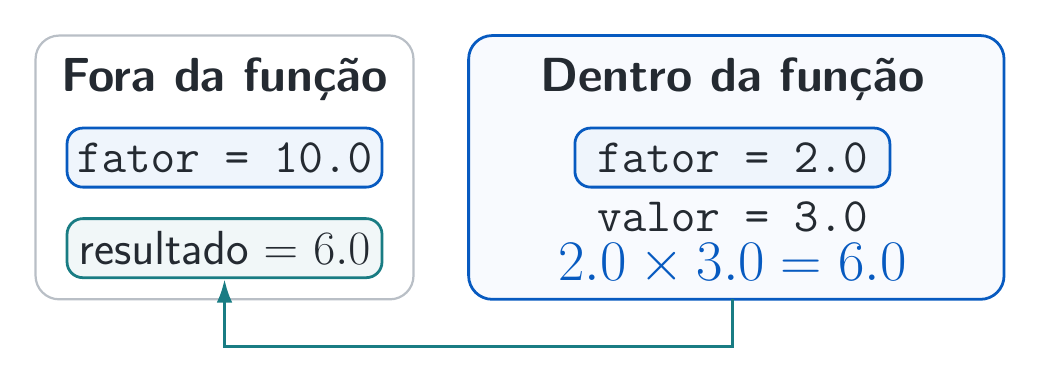
\begin{tikzpicture}[
  x=1cm,y=1cm,every node/.append style={font=\sffamily\fontsize{17}{21}\selectfont},
  valor/.style={draw=lnccblue,fill=lightblue,rounded corners=2mm,line width=1pt,
    align=center,minimum height=.75cm},
  seta/.style={-{Latex[length=3mm,width=2mm]},draw=teal,line width=1.2pt}
]
\path[use as bounding box] (-.1,-2.1) rectangle (12.4,2.15);
\draw[draw=muted!45,line width=.8pt,rounded corners=3mm] (0,-1.3) rectangle (4.8,2.05);
\draw[draw=lnccblue,line width=1pt,fill=lightblue!45,rounded corners=3mm] (5.5,-1.3) rectangle (12.3,2.05);
\node[text=ink,font=\sffamily\fontsize{18}{22}\selectfont\bfseries] at (2.4,1.5) {Fora da função};
\node[text=ink,font=\sffamily\fontsize{18}{22}\selectfont\bfseries] at (8.85,1.5) {Dentro da função};
\node[valor,minimum width=4.0cm] at (2.4,.5) {\texttt{fator = 10.0}};
\node[valor,draw=teal,fill=teal!6,minimum width=4.0cm] (resultado) at (2.4,-.65) {resultado = $6.0$};
\node[valor,minimum width=4.0cm] at (8.85,.5) {\texttt{fator = 2.0}};
\node[text=ink] at (8.85,-.25) {\texttt{valor = 3.0}};
\node[text=lnccblue,font=\sffamily\fontsize{20}{24}\selectfont] at (8.85,-.85) {$2.0\times3.0=6.0$};
\draw[seta] (8.85,-1.3) -- (8.85,-1.9) -- (2.4,-1.9) -- (resultado.south);
\end{tikzpicture}
\end{document}
